\section{Casi d'Uso}
\subsection{Introduzione}
In questa sezione sono presentati i casi d'uso che risultano rilevanti per il prodotto Personal Identity Wallet. 
Essi sono stati individuati e definiti attraverso l'analisi del capitolato d'appalto, gli incontri con il proponente e le riunioni interne del team Project Origin.
Ciascun caso d'uso rappresenta un insieme di scenari che hanno lo stesso obiettivo finale per un utente generico del sistema, definito \textbf{\textit{holder}}.
Le norme e le convenzioni adottate per la stesura di ogni caso d'uso sono descritte in dettaglio all'interno del documento Norme di Progetto.
 \subsection{Codice identificativo}
Ciascun caso d'uso viene categorizzato utilizzando la seguente notazione:
\begin{center}\begin{verbatim}
    CU{ID} - {Nome}
\end{verbatim}\end{center}
Ogni caso d’uso è inoltre definito secondo la seguente struttura:
\begin{itemize}
    \item \textbf{ID}: il codice del caso d’uso secondo la convenzione specificata precedentemente;
    \item \textbf{Nome}:  specifica il titolo del caso d’uso;
    \item \textbf{Attori}:  indica gli attori principali (ad esempio l’utente generico) e secondari (ad esempio entità di autenticazione esterne) del caso d’uso;
    \item \textbf{Precondizioni}:  specifica le condizioni che sono identificate come vere prima del verificarsi degli eventi del caso d’uso;
    \item \textbf{Postcondizioni}:  specifica  le  condizioni  che  sono  identificate  come  vere  dopo  il verificarsi degli eventi del caso d’uso;
    \item \textbf{Scenario  principale}:  rappresenta  il  flusso  degli  eventi,  a  volte  attraverso  l'uso di  una  lista  numerata;
    %\item \textbf{Inclusioni}:  usate per non descrivere più volte lo stesso flusso di eventi, inserendo il comportamento comune in un caso d’uso a parte;
\end{itemize}
Alcuni  casi  d’uso  possono  essere  associati  ad  un Diagramma UML  dei  casi  d'uso riportante lo stesso titolo e codice.
\subsection{Attori}
\begin{itemize}
    \item\textbf{Holder.}
    \item\textbf{Issuer.}
    \item\textbf{Verifier.}
\end{itemize}

\subsection{Elenco dei casi d'uso}
\subsubsection{UC01 - Richiesta di credenziali per Wallet}
\begin{itemize}
\item \textbf{Attore principale:} Holder.
\item \textbf{Attore secondario}: Issuer. 
\item \textbf{Precondizioni:} L’utente (\textit{holder}) non è in possesso delle credenziali.
\item \textbf{Postcondizioni:} L’utente (\textit{holder}) è riuscito a presentare la richiesta per la credenziale nel sito dell’ \textit{issuer} ed ora la sua richiesta deve essere esaminata.
\item \textbf{Scenario principale}: 
    \begin{enumerate}
        \item L' \textit{holder} deve richiedere delle credenziali; 
        \item l' \textit{holder} naviga nel sito dell' \textit{issuer}; 
        \item l' \textit{holder} presenta richiesta della credenziale che necessita; 
        \item l' \textit{holder} attende che la sua richiesta venga esaminata dall'\textit{issuer}.
    \end{enumerate}
\end{itemize}

\subsubsection{UC02 - Rilascio delle credenziali per Wallet}
\begin{itemize}
\item \textbf{Attore principale:} Issuer.
\item \textbf{Precondizioni:} L’ \textit{issuer} riceve una richiesta di credenziale.
\item \textbf{Postcondizioni:} L’ \textit{issuer} ha approvato la richiesta ed ha fornito la credenziale.
\item \textbf{Scenario principale:}
    \begin{enumerate}
        \item L' \textit{issuer} riceve una richiesta per rilasciare una credenziale; 
        \item l' \textit{issuer} approva la richiesta; 
    \end{enumerate}
\end{itemize}

\subsubsection{UC03 - Ottenimento delle credenziali per Wallet}
\begin{itemize}
\item \textbf{Attore principale:} Holder.
\item \textbf{Attore secondario:} Issuer.
\item \textbf{Precondizioni:} La credenziale è stata fornita dall' \textit{issuer}, l' \textit{holder} non è in possesso delle credenziali sul proprio Wallet.
\item \textbf{Postcondizioni:} l' \textit{holder} possiede all’interno del proprio Wallet la credenziale.
\item \textbf{Scenario principale:} 
    \begin{enumerate}
        \item L' \textit{holder} non è in possesso della credenziale;
        \item l' \textit{holder} salva la credenziale approvata dall' \textit{issuer} sul propio Wallet personale.
    \end{enumerate}
\end{itemize}
\begin{center}
    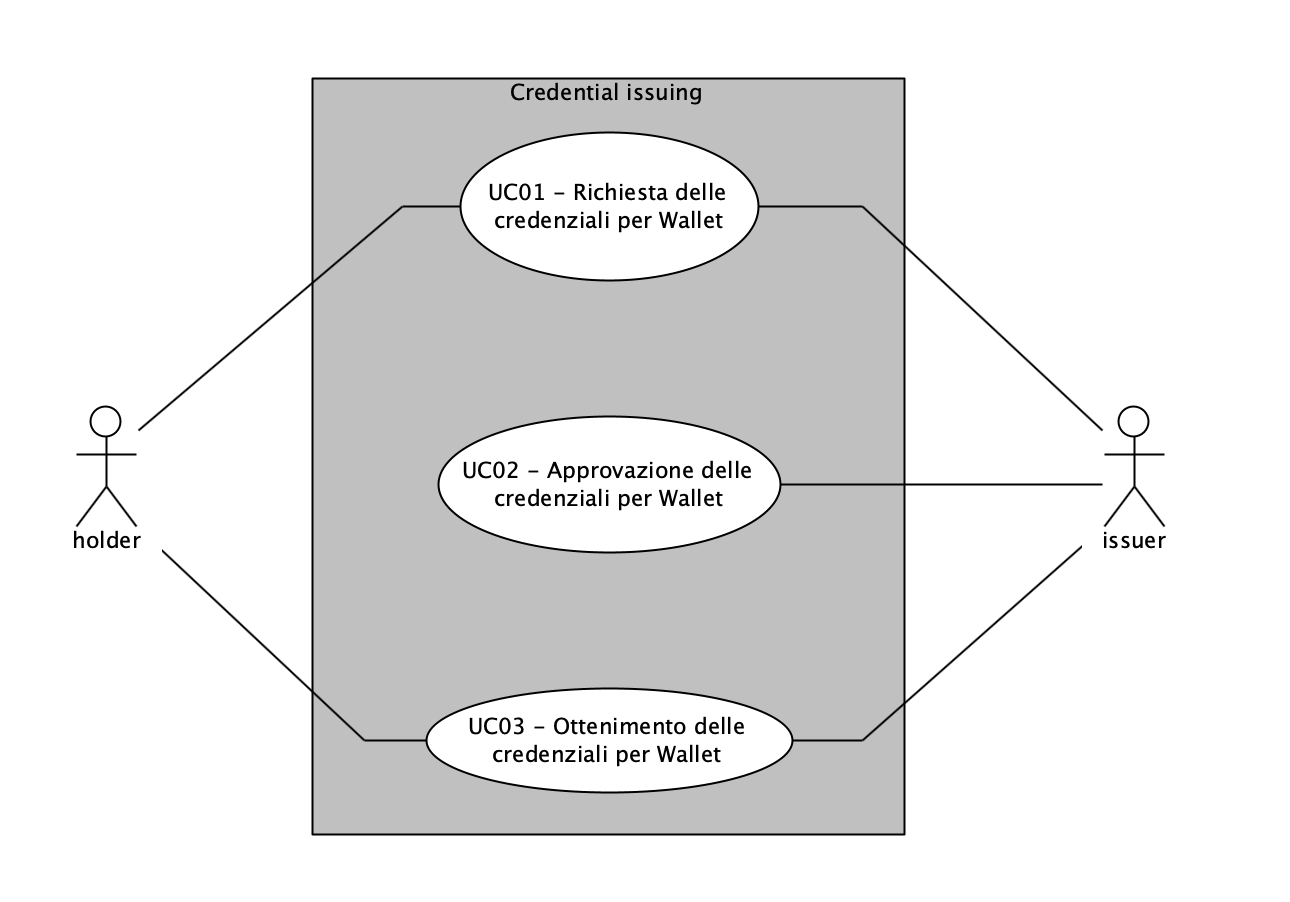
\includegraphics[scale = 0.65]{./res/img/credentialIssuing.png}
\end{center}

\subsubsection{UC04 - Visualizzazione delle credenziali}
\begin{itemize}
\item \textbf{Attore principale:} Holder.
\item \textbf{Precondizioni:} L’ \textit{holder} non ha ancora visualizzato la credenziale.
\item \textbf{Postcondizioni:} L’ \textit{holder} è riuscito a visualizzare la credenziale.
\item \textbf{Scenario principale:} 
    \begin{enumerate}
        \item L' \textit{holder} non ha visualizzato la credenziale; 
        \item l' \textit{holder} seleziona la credenziale nel proprio Wallet;
        \item l' \textit{holder} visualizza la credenziale.
    \end{enumerate}
\end{itemize}

\subsubsection{UC05 - Cancellazione delle credenziali}
\begin{itemize}
\item \textbf{Attore principale:} Holder.
\item \textbf{Precondizioni:} L’ \textit{holder} vuole rimuovere una credenziale dal Wallet personale.
\item \textbf{Postcondizioni:} L’ \textit{holder} è riuscito a rimuovere con successo la credenziale dal Wallet personale.
\item \textbf{Scenario principale:} 
    \begin{enumerate}
        \item L' \textit{holder} ha accesso al prprio Wallet personale; 
        \item l' \textit{holder} seleziona la credenziale nel proprio Wallet;
        \item l' \textit{holder} elimina la credenziale.
    \end{enumerate}
\end{itemize}
\begin{center}
    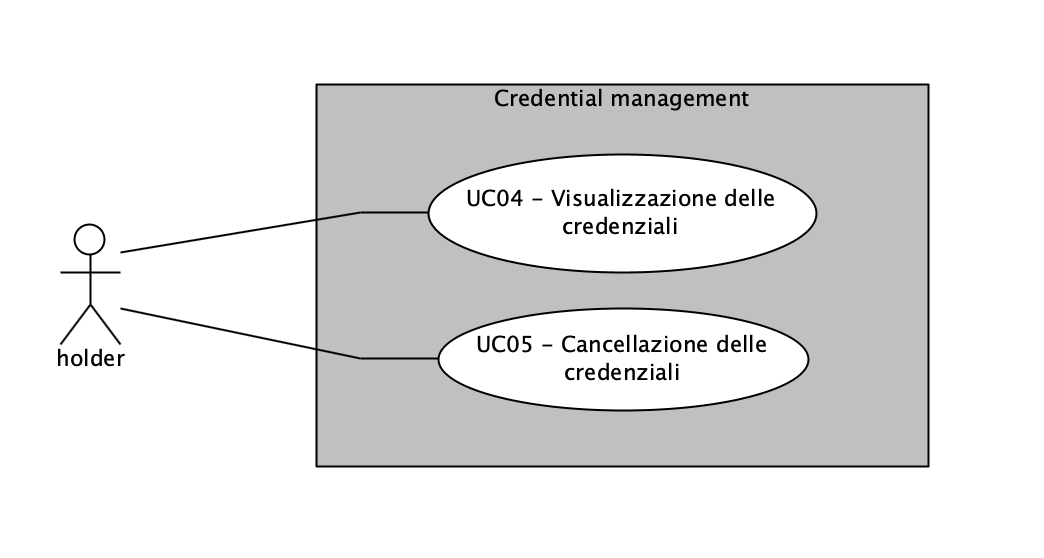
\includegraphics[scale = 0.65]{./res/img/credentialManagement.png}
\end{center}

\subsubsection{UC06 - Richiesta credenziali per verifica}
\begin{itemize}
\item \textbf{Attore principale:} Verifier.
\item \textbf{Attore secondario:} Holder; 
\item \textbf{Precondizioni:} Il \textit{verifier} deve richiedere una credenziale all' \textit{holder};
\item \textbf{Postcondizioni:} Il \textit{verifier} ha presentato una richiesta di una credenziale all' \textit{holder}.
\item \textbf{Scenario principale:} 
    \begin{enumerate}
        \item Il \textit{verifier} fa richiesta ad un \textit{holder} di fornirgli una credenziale salvata nel suo Wallet.
    \end{enumerate}
\end{itemize}

\subsubsection{UC07 - Fornitura delle credenziali per verifica}
\begin{itemize}
\item \textbf{Attore principale:} Holder. 
\item \textbf{Attore secondario:} Verifier.
\item \textbf{Precondizioni:} L’ \textit{holder} vuole fornire la credenziale presente nel Wallet personale al \textit{verifier}.
\item \textbf{Postcondizioni:} La credenziale dell’ \textit{holder} è stata fornita al \textit{verifier}.
\item \textbf{Scenario principale:} 
    \begin{enumerate}
        \item L' \textit{holder} fornisce al \textit{verifier} la credenziale che gli è stata richiesta.
    \end{enumerate}
\end{itemize}
\begin{center}
    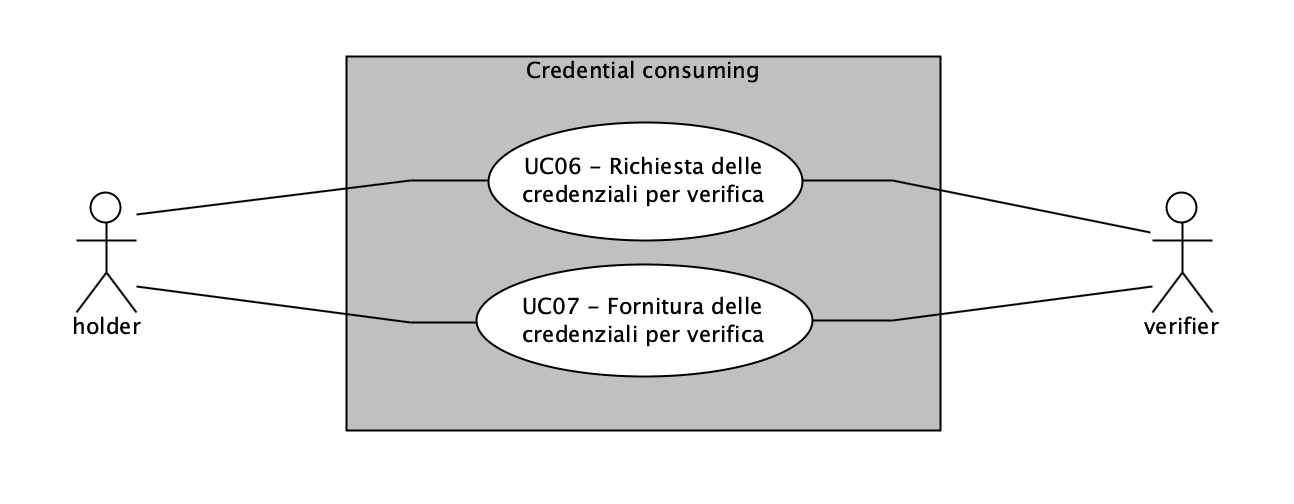
\includegraphics[scale = 0.65]{./res/img/credentialConsuming.png}
\end{center}
